\chapter{Pitch Detection}
\label{pitch-detection}

Pitch detection is simply frequency detection with the restriction of note quantization,
\autoref{notes-frequencies} shows the base frequency for each of the 12 existent
notes. Multiples of the same frequency are seen as the same note on a different
range, known as octave.

\begin{table}[htb]
  \begin{center}
    \ABNTEXreducedfont
    \caption[Notes Frequencies]{Notes Frequencies}
    \label{notes-frequencies}
    \begin{tabular}{c|c}
      \hline
      Note Name & Frequency\\
      \hline
      A & 440.00 \\
      A\# & 466.16 \\
      B & 493.88 \\
      C & 523.25 \\
      C\# & 554.37 \\
      D & 587.33 \\
      D\# & 622.25 \\
      E & 659.25 \\
      F & 698.46 \\
      F\# & 739.99 \\
      G & 783.99 \\
      G\# & 830.61 \\
      \hline
    \end{tabular}
    \legend{Source: made by authors}
  \end{center}
\end{table}

Even though the quantization makes things simpler it's still a hard task, even
more for instruments where there is the presence of harmonic series. Harmonic
series notes are multiples of the fundamental frequency (most important
note) produced by integer sections of the instrument vibration. \autoref{harmonic-series}
shows an visual representation of why there exist. The existence of them as well
as the presence of both inter-signal and white noise makes necessary the use of
non-trivial algorithms for pitch detection, and two of them will be discussed next.

\begin{figure}[htb]
	\caption{Harmonic Series}
  \label{harmonic-series}
	\begin{center}
    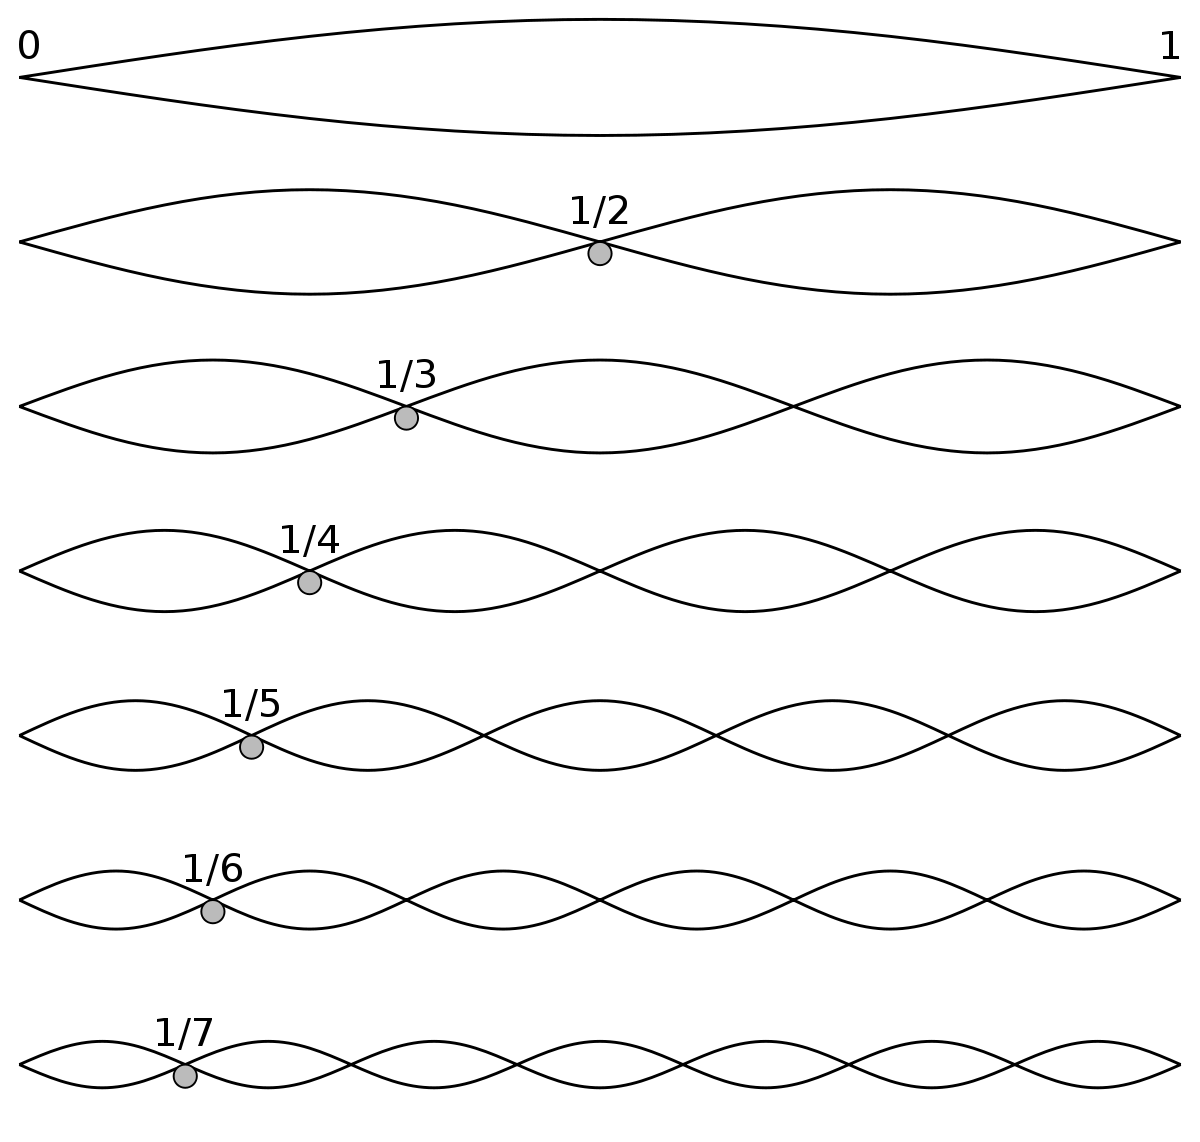
\includegraphics[scale=0.15]{images/harmonic-series.png}
	\end{center}
  \legend{Source: \citeonline{harmonic-series-figure-source}}
\end{figure}

\section{YIN algorithm}
Autocorrelation is a well know function to calculate a signal's fundamental
frequency, but it gives too much error for this project use case. YIN \cite{YINArticle}
is a method that uses a few improvements to the autocorrelation method, achieving
a much higher precision. It also can be implemented with logarithmic growth as the
autocorrelation can be calculated using the fft and ifft algorithms. The algorithm
can be divided in 6 steps, as follows:

\begin{enumerate}
  \item Autocorrelation
  \item Difference
  \item Cumulative mean normalized difference
  \item Absolute threshold
  \item Parabolic interpolation
  \item Best local estimate
\end{enumerate}

It's important to notice that the absolute threshold is a controlled attempt to regulate
the error introduced by the harmonic series (as in \autoref{harmonic-series}),
it thus gives preference to lower frequencies (below the threshold).

\section{MacLeod algorithm}
MacLeod \cite{MacLeodArticle} goes for another approach, using the square difference
function. More precisely it uses a special normalized version of it. The best result
is then calculated by means of using a parabolic interpolation of the highest
peak and its two neighbors, this process also gives a threshold constant that limits
the detection of the neighbors, thus the possibility of some tuning. As we will
see this gave the best results for our project after some tuning.

\section{Implementation}
